\title{BoG-2015-Poster}
%%%%%%%%%%%%%%%%%%%%%%%%%%%%%%%%%%%%%%%%%
% a0poster Portrait Poster
% LaTeX Template
% Version 1.0 (22/06/13)
%
% The a0poster class was created by:
% Gerlinde Kettl and Matthias Weiser (tex@kettl.de)
% 
% This template has been downloaded from:
% http://www.LaTeXTemplates.com
%
% License:
% CC BY-NC-SA 3.0 (http://creativecommons.org/licenses/by-nc-sa/3.0/)
%
%%%%%%%%%%%%%%%%%%%%%%%%%%%%%%%%%%%%%%%%%

%----------------------------------------------------------------------------------------
%	PACKAGES AND OTHER DOCUMENT CONFIGURATIONS
%----------------------------------------------------------------------------------------

\documentclass[a0,landscape]{a0poster}
\usepackage{multicol} % This is so we can have multiple columns of text side-by-side
\columnsep=100pt % This is the amount of white space between the columns in the poster
\columnseprule=3pt % This is the thickness of the black line between the columns in the poster

\usepackage{color}
 
\definecolor{sangertext}{RGB}{7,73,135}
\definecolor{sangersubtitletext}{RGB}{106,185,215}
\definecolor{codepurple}{rgb}{0.58,0,0.82}
\definecolor{backcolour}{rgb}{0.95,0.95,0.92}

\usepackage[scaled=.90]{helvet}

\usepackage{graphicx} % Required for including images
\graphicspath{{figures/}} % Location of the graphics files
\usepackage{booktabs} % Top and bottom rules for table
\usepackage[font=small,labelfont=bf]{caption} % Required for specifying captions to tables and figures
\usepackage{subcaption}
\usepackage{amsfonts, amsmath, amsthm, amssymb} % For math fonts, symbols and environments
\usepackage{wrapfig} % Allows wrapping text around tables and figures
\usepackage{enumerate}
\usepackage[hyphens]{url}
\usepackage{sidecap}
\usepackage[colorlinks,urlcolor=red,linkcolor=black,citecolor=black,linktoc=all]{hyperref}
\setlength{\columnseprule}{0.01pt}
\renewcommand{\columnseprulecolor}{\color[rgb]{0.9,0.9,0.9}}

\renewcommand{\familydefault}{\sfdefault}

\setlength\heavyrulewidth{0.1pt}
\setlength\lightrulewidth{0.1pt}

\usepackage{sectsty}
\sectionfont{\color{sangertext}}
\subsectionfont{\color{sangersubtitletext}}

\usepackage[square,numbers]{natbib}

\begin{document}

%----------------------------------------------------------------------------------------
%	POSTER HEADER 
%----------------------------------------------------------------------------------------

\begin{minipage}[b]{0.80\linewidth}
\veryHuge \color{sangertext} \textbf{64,976 whole genome haplotypes from the Haplotype Reference Consortium\\and efficient algorithms to use them} \color{sangersubtitletext}\\ % Title
\Large \color{black} \textbf{Richard M. Durbin}\textsuperscript{1}, Warren Kretzschmar\textsuperscript{2}, Shane A. McCarthy\textsuperscript{1}, Sayantan Das\textsuperscript{3}, Petr Dan\v{e}\v{c}ek\textsuperscript{1}, Christian Fuchsberger\textsuperscript{3},Olivier Delaneau\textsuperscript{4}, Hyun Min-Kang\textsuperscript{3},\\Gon\c{c}alo Abecasis\textsuperscript{3}, Jonathan Marchini\textsuperscript{2} on behalf of the Haplotype Reference Consortium\\[0.cm] % Author(s)
\large \textsuperscript{1}Wellcome Trust Sanger Institute, Hinxton, Cambridgeshire, CB10 1SA, UK
       \textsuperscript{2}Wellcome Trust Centre for Human Genetics, University of Oxford, Oxford, OX3 7BN, UK\\
       \textsuperscript{3}Department of Biostatistics and Center for Statistical Genetics, University of Michigan, Ann Arbor, MI 48109
       \textsuperscript{4}D\'{e}partement de G\'{e}n\'{e}tique et D\'{e}veloppement, Facult\'{e} de M\'{e}decine, Universit\'{e} de Gen\'{e}ve, Geneva, Switzerland\\[0.4cm]
\end{minipage}
\hspace{-4cm}
\begin{minipage}[b]{0.35\linewidth}

\includegraphics[width=24cm]{images/logos2.pdf}\\
\vspace{2.5cm}
\end{minipage}

\vspace{-1.75cm}
\begin{center}\noindent\rule{112cm}{0.01pt}\end{center}

%----------------------------------------------------------------------------------------

\begin{multicols}{3}

%----------------------------------------------------------------------------------------
%	INTRODUCTION
%----------------------------------------------------------------------------------------

\section*{Introduction}

Genotype imputation infers missing genotypes in samples from a reference panel, so can fill in full sequences from genome-wide association study (GWAS) data.
It is central to modern genetic association studies, supporting meta-analysis and increasing coverage and power.
The Haplotype Reference Consortium (HRC) has combined whole genome sequence data from \textbf{32,488 samples} from 20 studies to build an imputation reference panel at \textbf{39,235,157 single nucleotide variant sites} with allele frequencies down to 0.01\% (1/10,000).
We provide internet-accessible servers for imputation from whole genome genotype data, and show that we can impute at the same accuracy sites with up to an order of magnitude lower allele frequency than 1000 Genomes Phase 3.

We also describe \texttt{pbwt} \cite{durbin2014efficient}, a new extremely rapid and scalable imputation software using the positional Burrows-Wheeler transform (PBWT).

%----------------------------------------------------------------------------------------
%	HRC
%----------------------------------------------------------------------------------------
\vspace{-0.5cm}

\section*{The Haplotype Reference Consortium Release 1}

%----------------------------------------------------------------------------------------
%	Contributing datasets
%----------------------------------------------------------------------------------------

\subsection*{Contributing datasets}

This first release of the Haplotype Reference Consortium reference panel (HRC.r1) combines data from 20 large whole-genome sequencing projects.
The majority of these cohorts consist of samples of European origin making the panel particularly suitable for imputing into samples of European ancestry.
\begin{center}\vspace{0.5cm}
{\small
\setlength{\tabcolsep}{32pt}
\captionsetup{type=table}
\begin{tabular}{l c c c}
\toprule
\textbf{Cohort} & \textbf{Samples} & \textbf{Avg. coverage} & \textbf{Nationality}\\
\midrule
UK10K & 3,715 & 6.5$\times$ & UK\\
Sardinia & 3,445 & 4$\times$ & Italy\\
IBD & 4,478 & 4$\times$/2$\times$ & UK\\
GoT2D & 2,710 & 4$\times$ + Exome & US\\
BRIDGES & 2,487 & 6-12$\times$ & US\\
1000 Genomes Phase 3 & 2,495 & 4$\times$ + Exome & Various\\
GoNL & 748 & 12$\times$ & Netherlands\\
AMD & 3,222 & 4$\times$ & US\\
HUNT & 1,023 & 4$\times$ & US\\
SiSu + Kuusamo & 1,918 & 4$\times$ & Finland\\
INGI-FVG & 250 & 4-10$\times$ & Italy\\
INGI-Val Borbera & 225 & 6$\times$ & Italy\\
MCTFR & 1,325 & 10$\times$ & US\\
HELIC & 247 & 4$\times$/1$\times$ & Greece\\
ORCADES & 398 & 4$\times$ & UK, Orkney\\
inCHIANTI & 676 & 7$\times$ & UK\\
GECCO & 1,131 & 4-6$\times$ & US\\
GPC & 697 & 30$\times$ & US\\
ProjectMinE & 935 & 45$\times$ & Netherlands\\
NEPTUNE & 403 & 4$\times$ & US\\
\midrule
 & \textbf{32,488} & & \\
\bottomrule
\end{tabular}
\captionof{table}{\color{black} Cohorts contributing to the HRC.r1 reference panel.}
}
\end{center}\vspace{0.05cm}

%----------------------------------------------------------------------------------------
%	Data Processing
%----------------------------------------------------------------------------------------
\vspace{-1.5cm}
\subsection*{Data Processing}

\begin{itemize}
\setlength{\itemsep}{1pt}
\renewcommand{\labelitemi}{$\rightarrow$} 
\item Take initial calls from each cohort.
\item Select calls with overall minor allele count (MAC)$\ge$5 and carry out cross cohort QC/consistency, removing some sites and samples (see Figure \ref{filtering}).
\item Obtain genotype likelihoods (GLs) at these sites from the original BAMs using SAMtools.
\item Recall haplotypes from GLs using a modified version of SNPtools \cite{wang2013integrative} that restricts the parental haplotype search based on the original haplotypes.
\item Finally re-phase with SHAPEIT and remove sites with MAC$<$5 in new call set.
\end{itemize}

\begin{center}\vspace{0.001cm}
\captionsetup{type=figure}
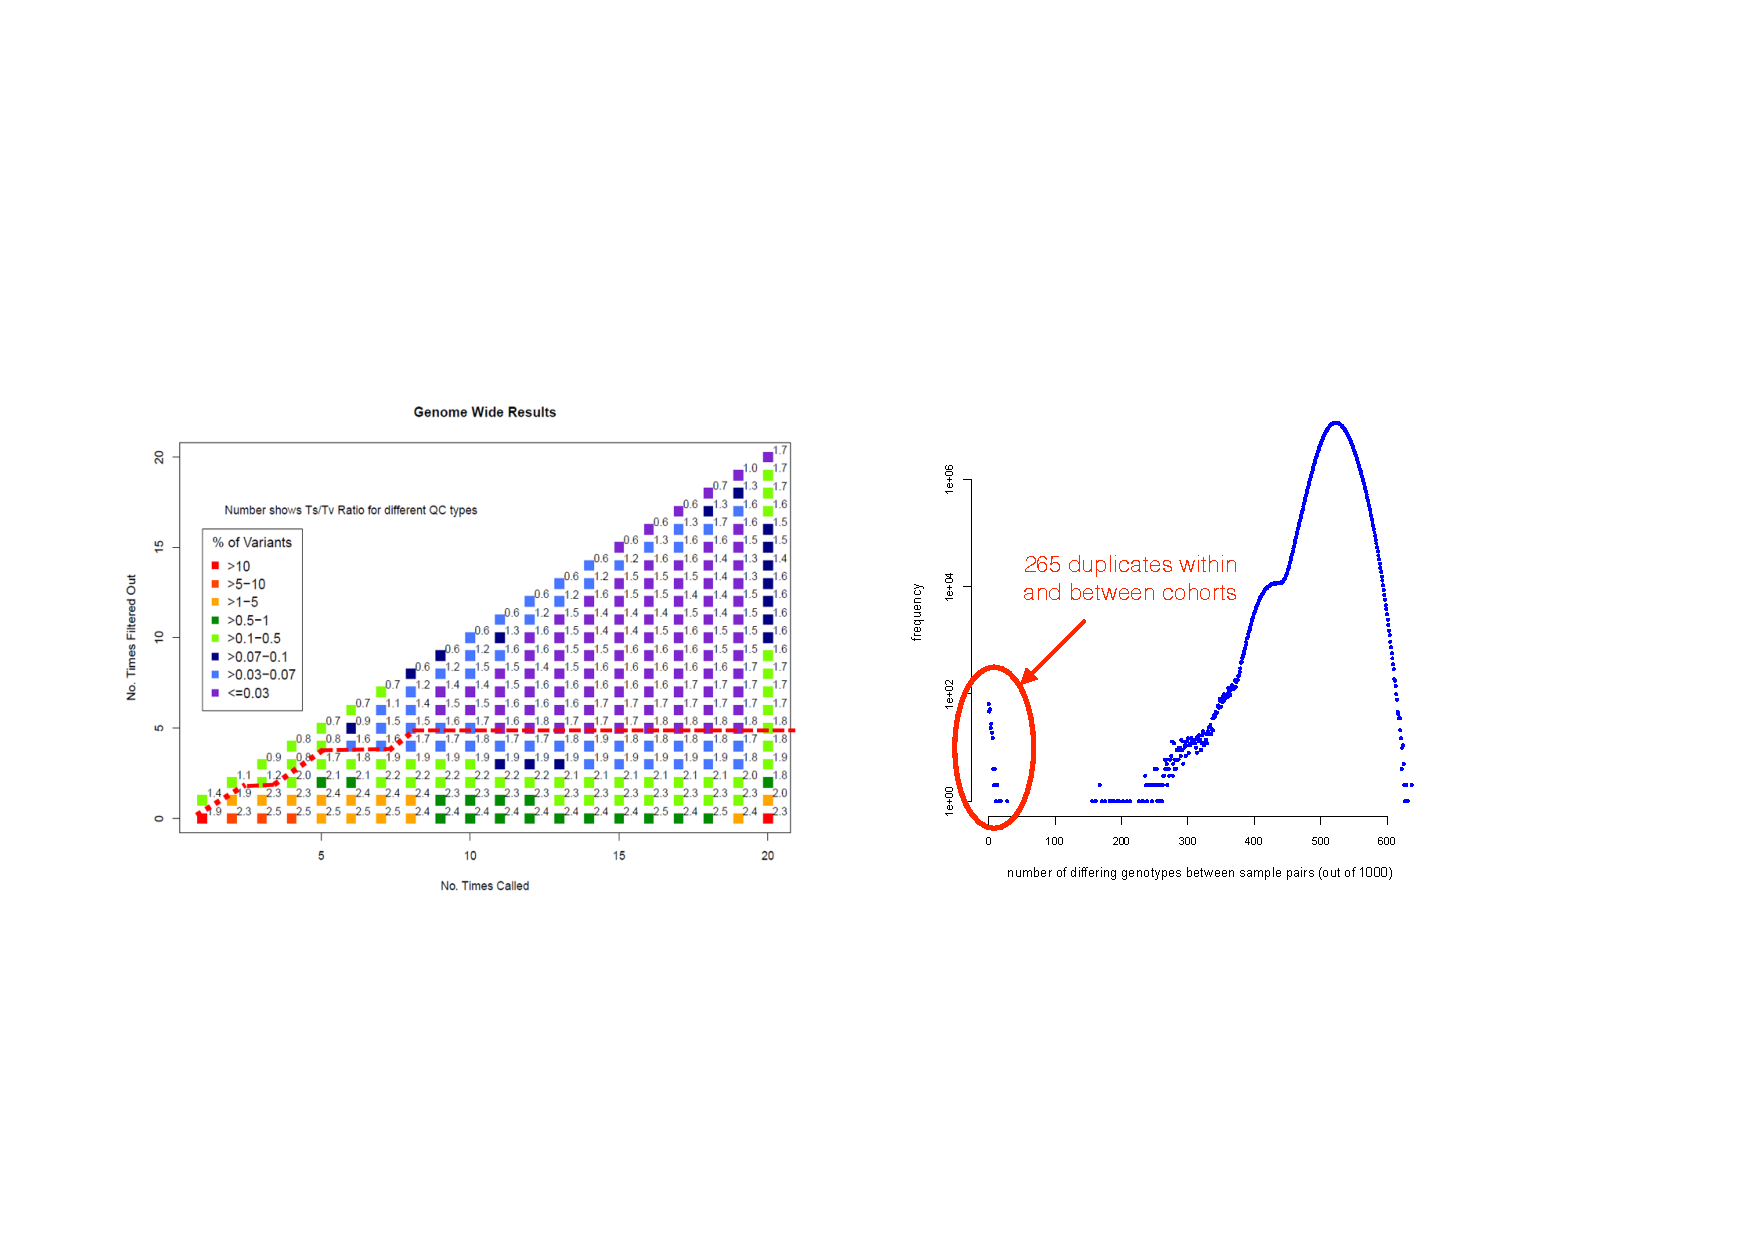
\includegraphics[width=0.7\linewidth]{images/filtering.pdf}
\captionof{figure}{\color{black}\textbf{Site and sample filtering}. Left: One site filter was to remove sites filtered out by 5 or more of the original cohorts (fewer if originally called in fewer); Right: we removed 265 duplicate samples.}
\label{filtering}
\end{center}\vspace{0.001cm}

\vfill
\columnbreak

%----------------------------------------------------------------------------------------
%	Imputation performance
%----------------------------------------------------------------------------------------

\subsection*{Improved imputation performance over existing panels}

\begin{center}\vspace{0.001cm}
\captionsetup{type=figure}
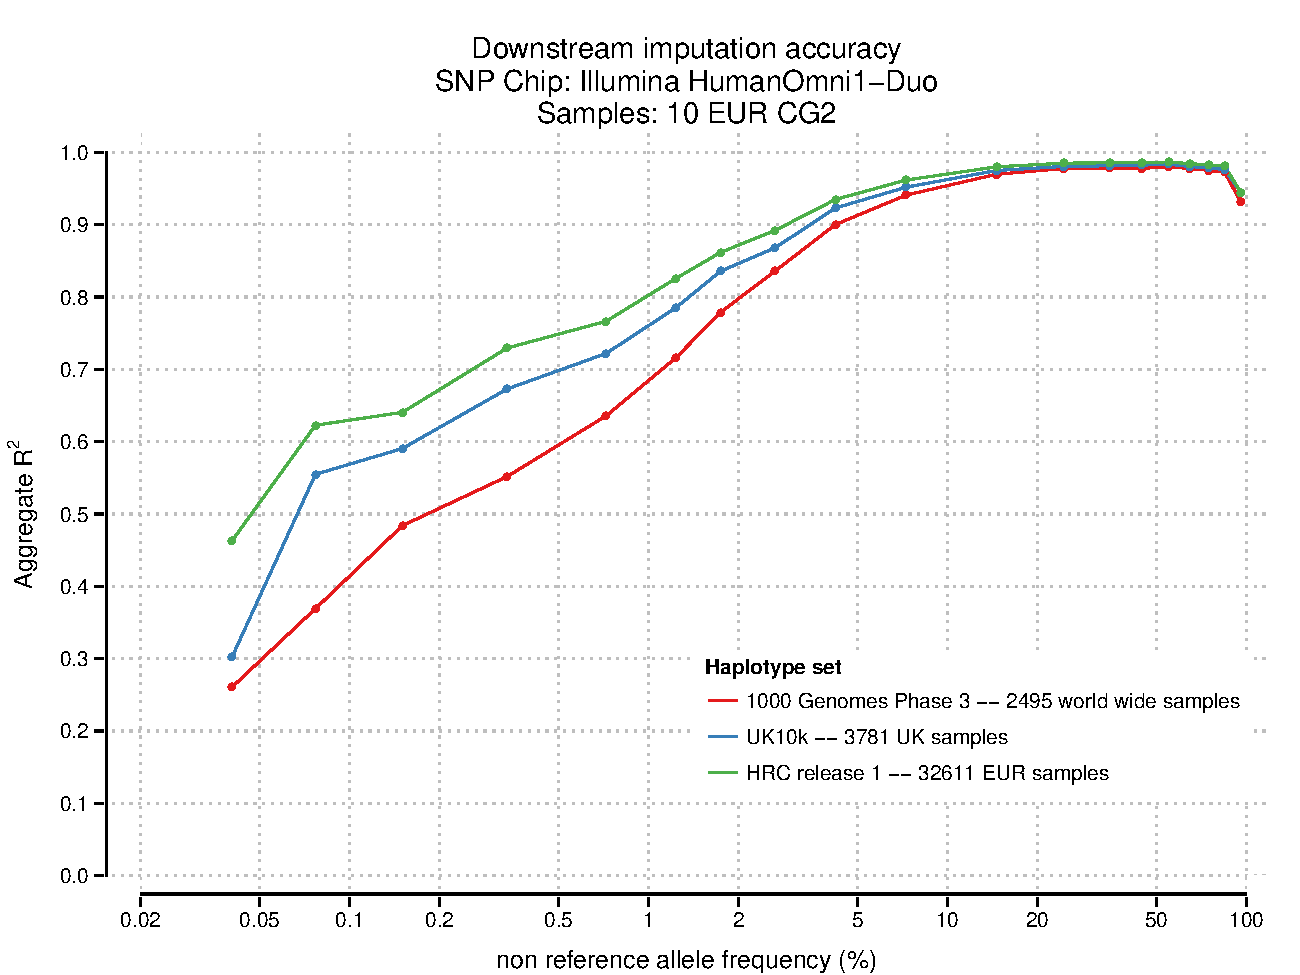
\includegraphics[width=0.7\linewidth]{images/bog20150430.pdf}
\captionof{figure}{\color{black}\textbf{Imputation performance on various panels}.
Pseudo-GWAS genotypes created by selecting genotypes at Illumina HumanOmni1−Duo chip sites from chromosome 20 of 10 CEU deep sequenced samples.
Imputation evaluated by comparing  high coverage genotype calls not in the selected chip sites with those imputed from the various panels using IMPUTE2.}
\end{center}\vspace{0.001cm}

\begin{itemize}
\setlength{\itemsep}{1pt}
\renewcommand{\labelitemi}{$\rightarrow$} 
\item HRC.r1 provides substantial increase over 1000 Genomes Phase 3 imputation (5-10$\times$ lower MAF).
\item Improvement over UK10K and other large single study panels while also greatly increasing the density of imputable sites ($\sim$22M for UK10K to $\sim$40M for HRC.r1).
\end{itemize}


\subsection*{Using the resource}

Making the full reference panel publicly available is not possible at the moment due to restrictions on data access, so we are making the panel available to users via \textbf{public imputation servers} at the Sanger Institute and at the University of Michigan.
Users upload phased or unphased GWAS data and imputed genotypes and dosages are returned.

The imputation engine used at the Sanger Institute is \texttt{pbwt} (see final section of this poster), while at the University of Michigan it is \texttt{minimac3} \cite{fuchsberger2014minimac2}.
Both servers optionally pre-phase GWAS data before imputation using SHAPEIT2 \cite{delaneau2013improved}.

\begin{center}\vspace{0.001cm}
\captionsetup{type=figure}
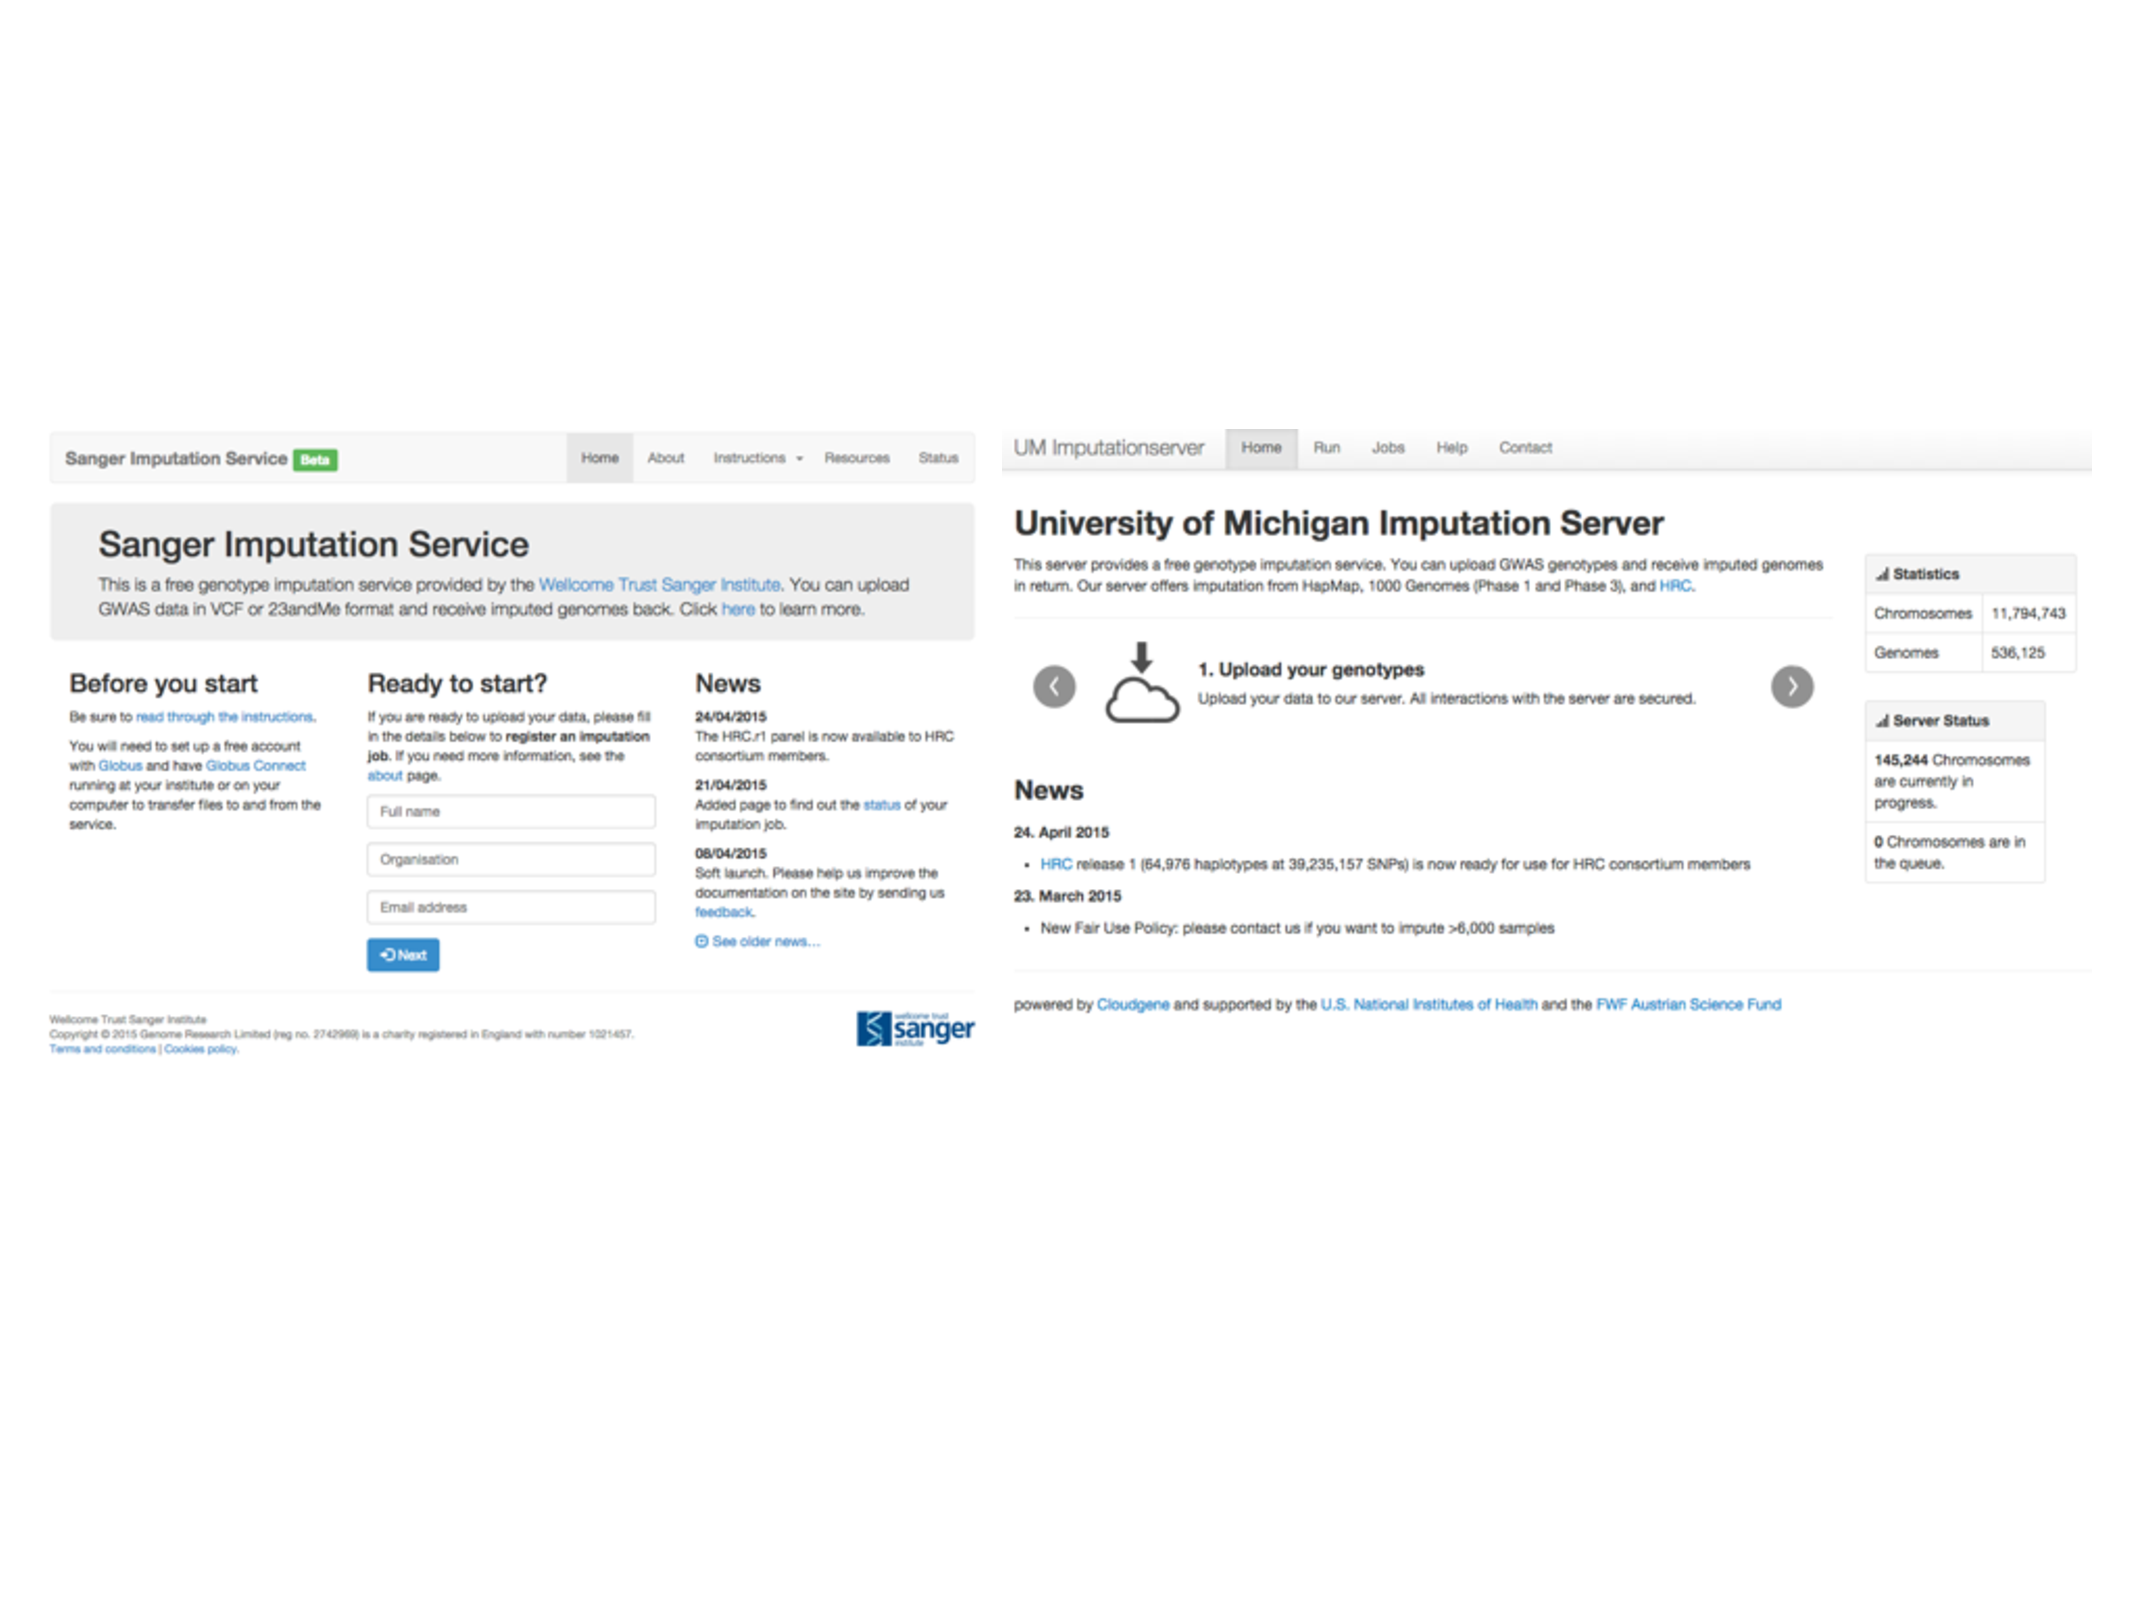
\includegraphics[width=0.9\linewidth]{images/servers.pdf}
\captionof{figure}{\color{black}\textbf{Imputation servers}. Left: the Sanger Institute server (\texttt{imputation.sanger.ac.uk}) uses \texttt{pbwt}. Right: The University of Michigan server (\texttt{imputationserver.sph.umich.edu}) uses \texttt{minimac3}.}
\end{center}\vspace{0.001cm}

\textbf{The HRC.r1 panel is currently available via the imputation servers to HRC contributors and will be available openly to all on July 1st.}

%----------------------------------------------------------------------------------------
%	HRC Future Plans
%----------------------------------------------------------------------------------------

\subsection*{HRC Future Plans}

\begin{description}
\item[Chromosome X] The currently available panel only contains the autosomes. We are currently working on adding in chromosome X.
\item[Availability in the EGA] We intend to deposit a subset of data in EGA with managed access for imputation only.
\item[GRCh38] We are planning to provide a GRCh38 version by liftover in the first instance.
\item[Release 2] Later in 2015 we will begin building release 2 with more data representing more populations outside of Europe including Africa, Asia and the Americas. If you have a cohort with sequencing data that you would like to see incorporated, please get in touch.
\end{description}

\vfill
\columnbreak

%----------------------------------------------------------------------------------------
%	Positional Burrows-Wheeler Transform (PBWT) and imputation
%----------------------------------------------------------------------------------------

\section*{Positional Burrows-Wheeler Transform (PBWT) and imputation}

The positional Burrows-Wheeler transform (PBWT) provides a compressed representation of a haplotype panel in which variant calls are implicitly available in sorted order at each site, sorted based on the preceding sequence \cite{durbin2014efficient}. The entire PBWT data for HRC release 1 is 3.9GB at 0.0015 bytes per genotype, compared to 70GB for the gzipped \texttt{.hap} files used by IMPUTE2.  

\begin{center}\vspace{0.001cm}
\captionsetup{type=figure}
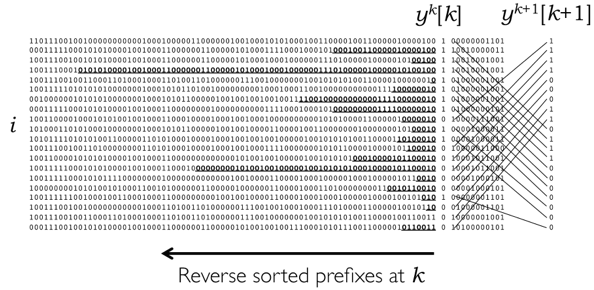
\includegraphics[width=0.7\linewidth]{images/pbwt2.png}
\captionof{figure}{\color{black}Procedure for updating the sort order and deriving the PBWT.}
\end{center}\vspace{0.001cm}

\noindent This structure also supports very fast exact matching of new sequences to find optimal local matches in the panel, in a manner equivalent to Burrows-Wheeler transform based matching in read aligners such as \texttt{bwa}.  We have developed a fast imputation algorithm by first finding, for each phased input haplotype, locally maximal matches to the observed data, then imputing missing values by taking a weighted sum of the values on the local matches. This is implemented in the \texttt{pbwt} package and can be used as\\
\texttt{pbwt -readVcfGT INPUT.vcf.gz -referenceImpute PANEL -writeVcfGz OUTPUT.vcf.gz}.

\begin{center}\vspace{0.001cm}
\captionsetup{type=figure}
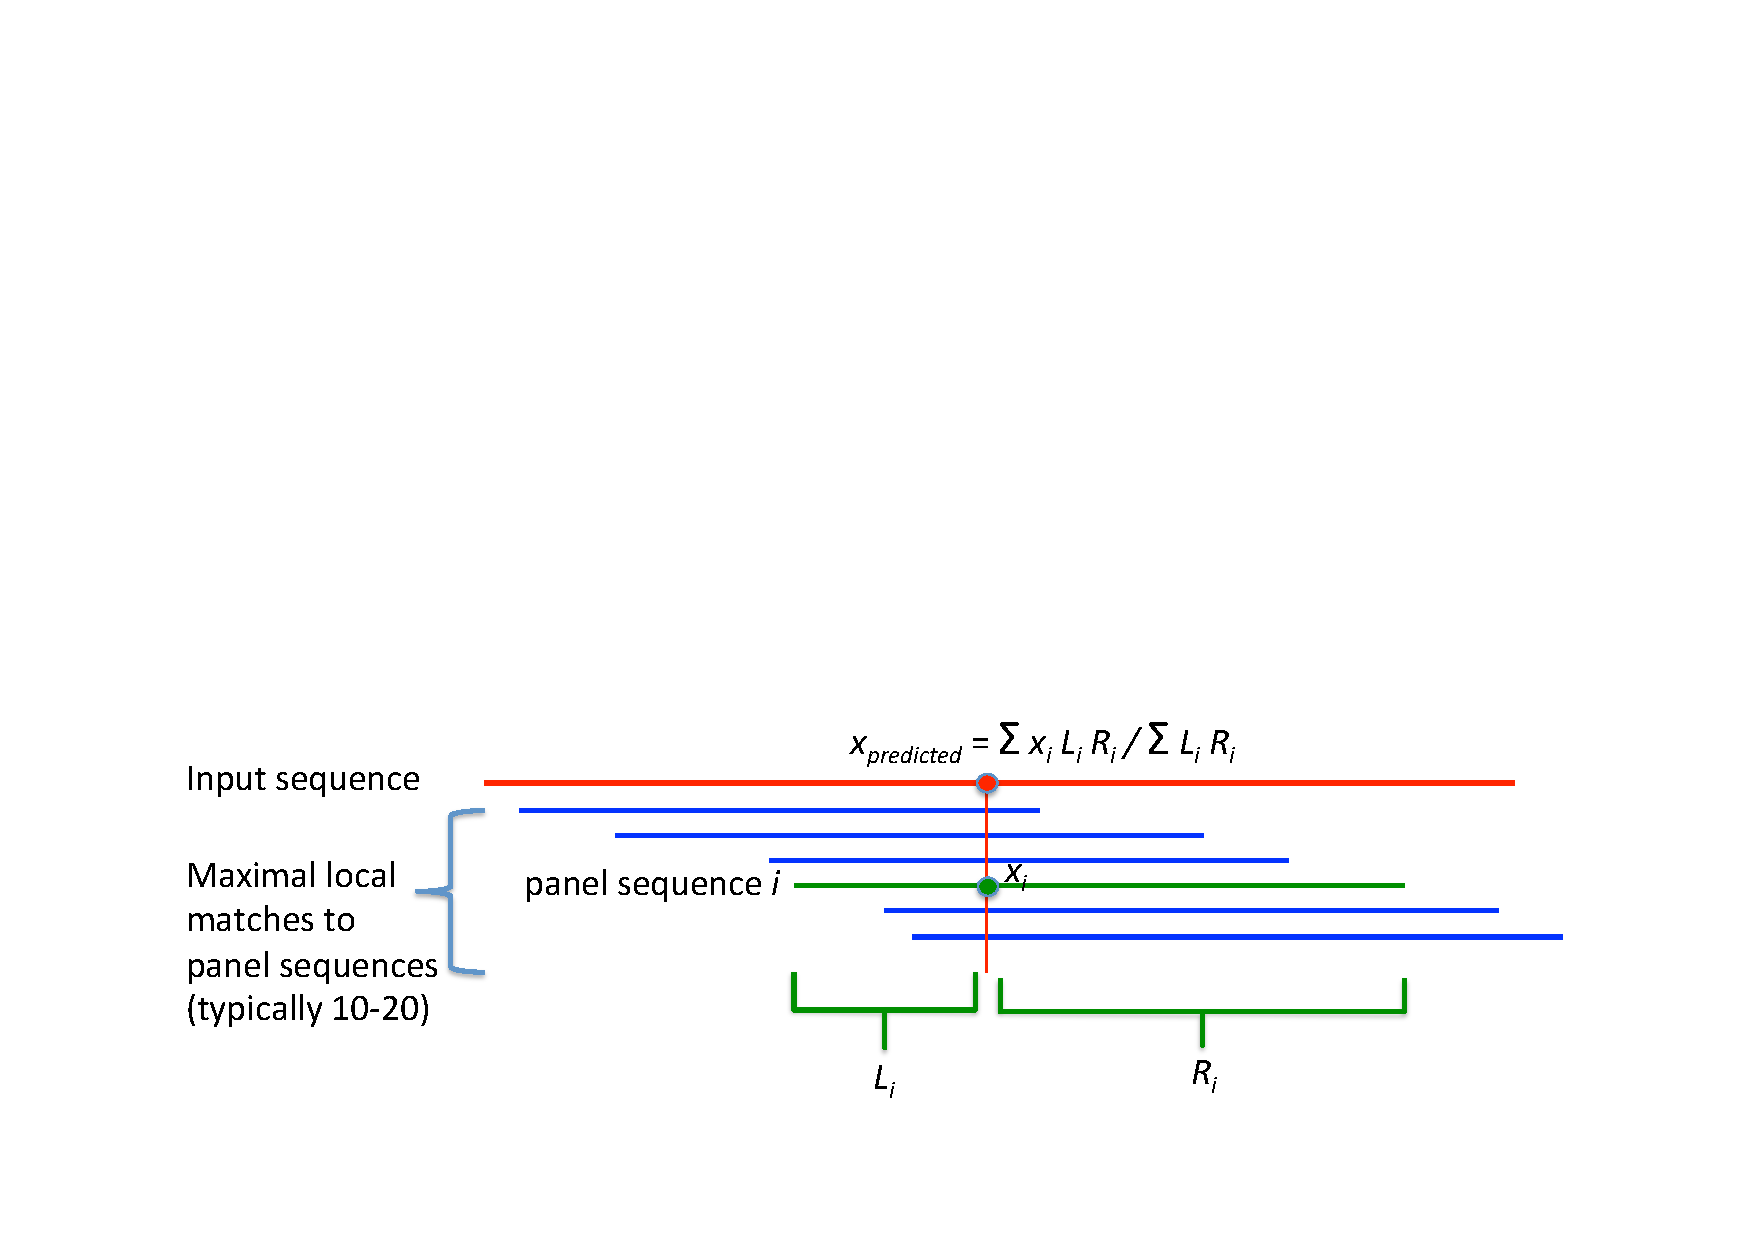
\includegraphics[width=0.6\linewidth]{images/matching.pdf}
\captionof{figure}{\color{black}Imputation based on local maximal haplotype matching.}
\end{center}\vspace{0.001cm}

\noindent This implementation can impute 1000 samples against HRC release 1 in on average 134 CPU seconds per sample, with 1.63GB memory requirement for chromosome 1 (imputation is split by chromosome), with accuracy a little lower than Minimac and IMPUTE2. 

\begin{center}\vspace{0.001cm}
\captionsetup{type=figure}
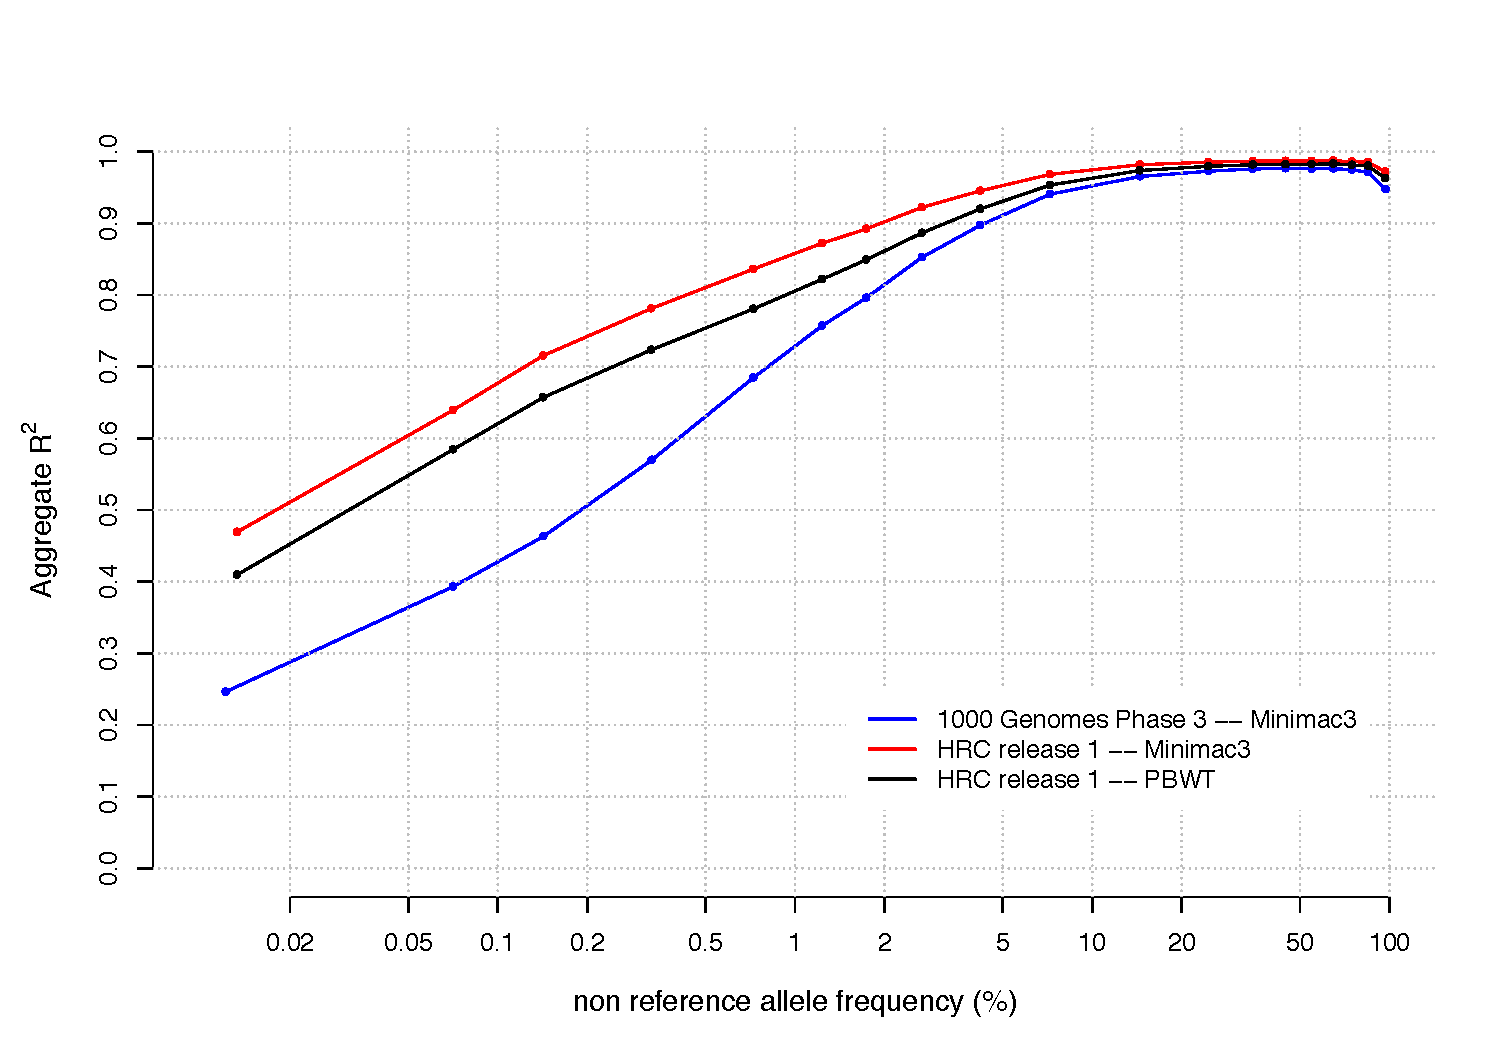
\includegraphics[width=0.6\linewidth]{images/HRC-G1K-Minimac-PBWT2.pdf}
\end{center}\vspace{0.001cm}

%----------------------------------------------------------------------------------------
%	REFERENCES
%----------------------------------------------------------------------------------------

\vspace{-2cm}

\bibliographystyle{unsrtnat}
\footnotesize
\setlength{\bibsep}{1pt}
\bibliography{hrc}

\begin{center}\vspace{0.5cm}
{\normalsize
\def\arraystretch{1.25}
\setlength{\tabcolsep}{12pt}
\begin{tabular}{r l}
\toprule
\textbf{Haplotype Reference Consortium} & \url{www.haplotype-reference-consortium.org}\\
\textbf{Sanger imputation server} & \url{imputation.sanger.ac.uk}\\
\textbf{UMich imputation server} & \url{imputationserver.sph.umich.edu}\\
\textbf{PBWT} & \url{github.com/richarddurbin/pbwt}\\
\textbf{Contact} & \href{mailto:richard.durbin@sanger.ac.uk}{\nolinkurl{richard.durbin@sanger.ac.uk}}\\
\bottomrule
\end{tabular}
}
\end{center}\vspace{0.05cm}


\end{multicols}
\end{document}